\let\lesson\undefined
\newcommand{\lesson}{\phantomlesson{Bài 11: Ba định luật Newton về chuyển động}}
\chapter[Định luật I Newton]{Định luật I Newton}
\setcounter{section}{0}
\section{Lý thuyết}
\subsection{Thí nghiệm của Galilei}
Galilei bố trí thí nghiệm như Hình \ref{fig:15.1}, rồi thả hòn bi cho lăn xuống theo máng nghiêng 1. Ông nhận thấy hòn bi lăn ngược lên máng 2 đến một độ cao thấp hơn độ cao ban đầu.
\begin{center}
	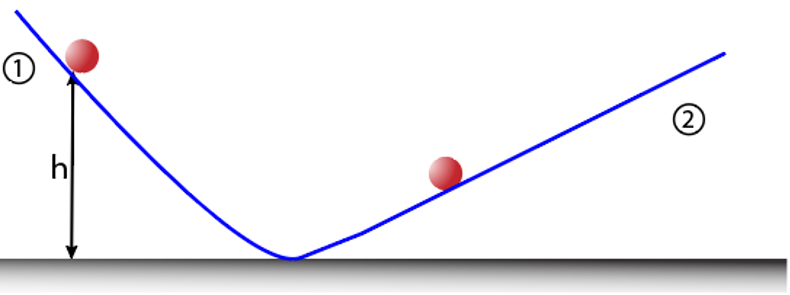
\includegraphics[width=0.3\linewidth]{../figs/VN10-2023-PH-TP015-1}
	\captionof{figure}{}
	\label{fig:15.1}
\end{center}
Khi hạ thấp độ nghiêng của máng 2, ông thấy hòn bi lăn trên máng 2 được một đoạn dài hơn. Ông cho rằng hòn bi không lăn được đến độ cao ban đầu là vì có ma sát.
\begin{center}
	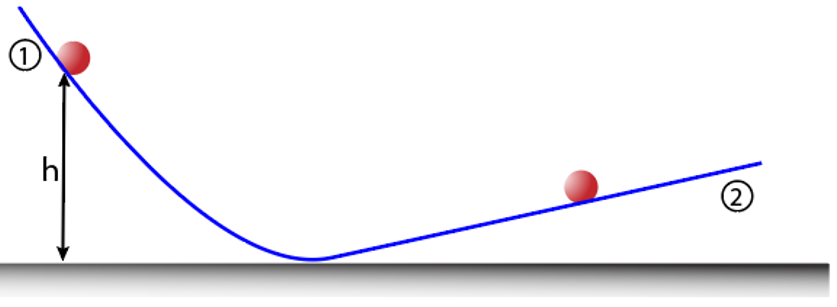
\includegraphics[width=0.3\linewidth]{../figs/VN10-2023-PH-TP015-2}
	\captionof{figure}{}
\end{center}
Ông tiên đoán rằng nếu không có ma sát và nếu máng nghiêng 2 nằm ngang thì hòn bi sẽ lăn mãi mãi với vận tốc không đổi.
\begin{center}
	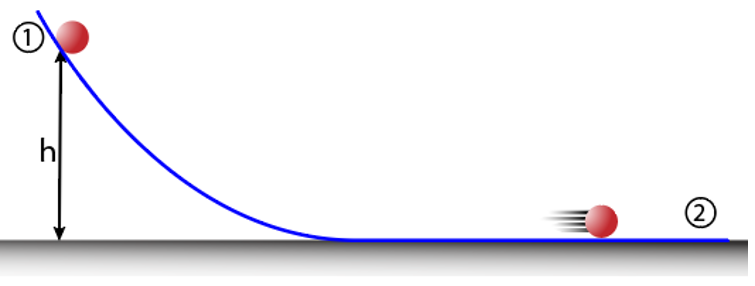
\includegraphics[width=0.3\linewidth]{../figs/VN10-2023-PH-TP015-3}
	\captionof{figure}{}
\end{center}
\subsection{Định luật I Newton}
\subsubsection{Phát biểu định luật}
Nếu một vật không chịu tác dụng của lực nào hoặc chịu tác dụng của các lực có hợp lực bằng không, thì vật đang đứng yên sẽ tiếp tục đứng yên, đang chuyển động sẽ tiếp tục chuyển động thẳng đều.
\luuy{Một vật nếu không chịu tác dụng của lực nào được gọi là vật tự do.}
\subsubsection{Ý nghĩa của định luật I Newton}
Lực không phải là nguyên nhanh gây ra chuyển động, mà là nguyên nhân làm thay đổi vận tốc chuyển động của vật.
\subsubsection{Quán tính}
Tính chất bảo toàn trạng thái đứng yên hay chuyển động của vật được gọi là quán tính của vật.
\begin{itemize}
	\item Do có quán tính mà mọi vật có xu hướng bảo toàn vận tốc cả về hướng về độ lớn.
	\item Định luật I được gọi là định luật quán tính và chuyển động thẳng đều được gọi là chuyển động theo quán tính.
	\item Hệ qui chiếu quán tính là hệ quy chiếu mà trong đó định luật 1 được nghiệm đúng. 
\end{itemize}
\section{Mục tiêu bài học - Ví dụ minh họa}
\begin{dang}{Ghi nhớ định luật I Newton. \\ Nhận biết quán tính}
	\viduii{1}
	{Một vật đang chuyển động với vận tốc $\SI{3}{\meter/\second}$ dưới tác dụng của các lực. Nếu bỗng nhiên các lực này mất đi thì:
	\begin{mcq}
		\item Vật dừng lại ngay.
		\item Vật đổi hướng chuyển động.
		\item Vật chuyển động chậm dần rồi dừng lại.
		\item Vật tiếp tục chuyển động theo hướng cũ với vận tốc $\SI{3}{\meter/\second}$.
\end{mcq}}
	{
\begin{center}
	\textbf{Hướng dẫn giải}
\end{center}	
Ban đầu vật đang chuyển động với vận tốc $\SI{3}{\meter/\second}$. Do đó, khi các lực tác dụng lên vật mất đi (vật tự do) thì vật sẽ tiếp tục chuyển động thẳng đều mãi mãi với vận tốc $\SI{3}{\meter/\second}$.\\
\textbf{Đáp án: D.}
}
	\viduii{2}{Một chiếc xe buýt đang chạy trên đường thì tài xế phanh xe gấp. Một hành khách ngồi ở cuối xe phàn nàn rằng, do bác tài xế phanh xe gấp mà chiếc túi xách ở phía trước bay về phía anh ta làm anh ta bị đau. Người hành khách nói đúng hay sai? Em hãy giải thích?
	}
	{	\begin{center}
			\textbf{Hướng dẫn giải}
		\end{center}
		
		Người hành khách đã nói sai. Khi xe dừng lại đột ngột, túi xách theo quán tính phải bay về phía trước, không phải bay về phía sau.
		
	}
\end{dang}	
\begin{dang}{Vận dụng định luật I Newton và quán tính}
	\viduii{2}
	{Đặt chiếc cốc đầy nước lên trên tờ giấy A4 đặt trên mặt bàn nhẵn và ở gần mép. Giật thật nhanh tờ giấy bằng một lực theo phương nằm ngang thì hiện tượng gì sẽ xảy ra với tờ giấy và cốc nước?
		\begin{center}
			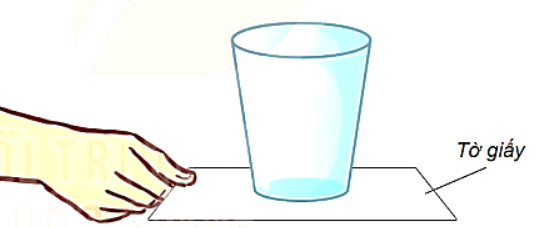
\includegraphics[width=0.3\linewidth]{../figs/VN10-2023-PH-TP015-4}
			\captionof{figure}{}
		\end{center}
	\begin{mcq}
		\item Tờ giấy chuyển động về một hướng, cốc nước chuyển động theo hướng ngược lại.
		\item Cốc nước chuyển động cùng với tờ giấy.
		\item Tờ giấy bị rút khỏi cốc nước mà nước vẫn không đổ.
		\item Tờ giấy bị đứt ở chỗ đặt cốc nước.
\end{mcq}}
	{\begin{center}
			\textbf{Hướng dẫn giải}
		\end{center}
	Tờ giấy bị rút khỏi cốc nước mà nước vẫn không đổ. Ban đầu cốc nước đang ở trạng thái đứng yên, khi rút nhanh tờ giấy, do quán tính nên cốc nước chưa kịp thay đổi trạng thái chuyển động của nó.\\
	\textbf{Đáp án: C.}
}
	\viduii{3}{\begin{enumerate}[label=\alph*.]
			\item Em hãy giải thích tại sao khi ta nhảy từ bậc cao xuống chân ta bị gập lại.  	
			\item Khi cán búa lỏng, tại sao ta có thể làm chặt lại bằng cách gõ mạnh đuôi cán xuống đất.
		\end{enumerate}
	}
	{	\begin{center}
			\textbf{Hướng dẫn giải}
		\end{center}
		
		\begin{enumerate}[label=\alph*.]
			\item Nhảy từ bậc cao xuống, chân chạm đất bị dừng lại ngay, nhưng người còn tiếp tục chuyển động theo quán tính nên làm chân gập lại.  	
			\item Khi gõ mạnh đuôi cán búa xuống đất, cán búa đột ngột dừng lại. Do quán tính đầu búa tiếp tục chuyển động gắn chặt vào cán búa. 
		\end{enumerate}
	}
\end{dang}
